\documentclass{article}

\usepackage[margin=0.5in,bottom=1in,footnotesep=1in]{geometry}

\usepackage{amsmath}


\usepackage{multicol}
\setlength{\columnsep}{1cm}
\usepackage[]{algorithm2e}

\usepackage{lipsum}% for dummy text
\usepackage[varg]{txfonts}
\usepackage{graphicx}
\usepackage{subcaption}
\usepackage{multirow}

\usepackage[font=small,labelfont={sf,bf}]{caption}


\usepackage{titlesec}
\titleformat{\section}{\fontfamily{phv}\fontsize{12}{15}\bfseries}{\thesection}{1em}{}
\titleformat{\subsection}{\fontfamily{phv}\fontsize{10}{15}\itshape}{\thesubsection}{1em}{}
\titleformat{\subsubsection}{\fontfamily{phv}\fontsize{9}{15}\bfseries}{\thesubsubsection}{1em}{}


\title{\textbf{FYS4150 Project 3: \\Numerical integration}}
\author{Marie Foss, Maria Hammerstr{{\o}}m}
\date{} % removes date from title

\begin{document}

\maketitle

\begin{abstract}
	\noindent We study the precision and efficiency of four different integration methods for a 6-dimensional integral with a known analytical solution: Gaussian quadrature using Legendre and Laguerre polynomials, and Monte Carlo integration with and without importance sampling. The Monte Carlo method \textit{with} importance sampling proved to be the superior method, both when it came to precision and speed. 
	%\lipsum[1]
	\vspace*{2ex}
	
	\noindent \textbf{Github:} \textit{https://github.com/mariahammerstrom/Project3}
	\vspace*{2ex}
\end{abstract}



\begin{multicols}{2}

\section{Introduction}
In this project we will determine the ground state correlation energy between two electrons in an helium atom by calculating a six-dimensional integral that appears in many quantum mechanical applications. The methods we will use are Gauss-Legendre and Gauss-Laguerre quadrature and Monte-Carlo integration. 

We assume that the wave function of each electron can be modelled like the single-particle wave function of an electron in the hydrogen atom. The single-particle wave function  for an electron $i$ in the $1s$ state  is given in terms of a dimensionless variable (the wave function is not properly normalized)

\begin{equation*}
	{\bf r}_i =  x_i {\bf e}_x + y_i {\bf e}_y +z_i {\bf e}_z ,
\end{equation*}
as

\begin{equation*}
	\psi_{1s}({\bf r}_i)  =   e^{-\alpha r_i},
\end{equation*}
where $\alpha$ is a parameter and 

\begin{equation*}
	r_i = \sqrt{x_i^2+y_i^2+z_i^2}.
\end{equation*}
We will fix $\alpha=2$, which should correspond to the charge of the helium atom $Z=2$. 

The ansatz for the wave function for two electrons is then given by the product of two 
so-called $1s$ wave functions as 

\begin{equation*}
	\Psi({\bf r}_1,{\bf r}_2)  =   e^{-\alpha (r_1+r_2)}.
\end{equation*}
The integral we need to solve is the quantum mechanical expectation value of the correlation energy between two electrons which repel each other via the classical Coulomb interaction, namely

\begin{equation}\label{eq:correlationenergy}
	\langle \frac{1}{|{\bf r}_1-{\bf r}_2|} \rangle = \int_{-\infty}^{\infty} \mathrm{d}{\bf r}_1\mathrm{d}{\bf r}_2  e^{-2\alpha (r_1+r_2)}\frac{1}{|{\bf r}_1-{\bf r}_2|}.
\end{equation}
In Cartesian coordinates, this integral can be rewritten as
\begin{equation}\label{eq:cartesian}
	\int\mathrm{d}\textbf{x}_1\mathrm{d}\textbf{x}_2\frac{\exp\left(-2\alpha\left[\sqrt{x_1^2+y_1^2+z_1^2}+ \sqrt{x_2^2+y_2^2+z_2^2}\right]\right)}{\left[(x_1-x_2)^2+(y_1-y_2)^2+(z_1-z_2)^2\right]^{1/2}},
\end{equation}
where $\mathrm{d}\textbf{x}_i=\mathrm{d}x_i\mathrm{d}y_i\mathrm{d}z_i$.


This integral can be solved in closed form, which gives an answer of $5\pi^2/16^2 \approx 0.192765710958777$.



\section{Methods}

\subsection{Gaussian quadrature}
Gaussian quadrature is a method that solves integrals with excellent results, giving high precision for few integration points compared to simpler integration methods such as Newton-Cotes quadrature. The basic idea behind the method is to approximate the given function by a polynomial of degree $2N-1$ so that

\begin{equation*}
	f(x) \approx P_{2N-1} (x),
\end{equation*}
where $P_{2N-1} (x)$ is a polynomial of degree $2N-1$ with only $N$ mesh points $x$. Gaussian quadrature says that we can calculate our integral in the following way:

\begin{equation}
	I = \int_a^b f(x) \mathrm{d}x = \int_a^b W(x) g(x) \mathrm{d}x \approx \sum_{i = 0}^{N-1} \omega_i g(x_i),
\end{equation}
where $\omega_i$ are the weights determined through the use of orthogonal polynomials, $W(x)$ is the weight function and $x_i$ are the chosen mesh points. $x_i$ will then be the zeros of these polynomials.

In this project we make use of Legendre and Laguerre polynomials to solve the integral in Eq. (\ref{eq:correlationenergy}). To know which polynomial to use we need to look at the weight function and interval for these polynomials to see which polynomial resembles our integral the most. For Legendre and Laguerre the weight functions and intervals are:

\begin{center}
\begin{tabular}{ l l l }\hline
	Polynomial 					& Interval	 				& Weight function		\\ \hline
	Legendre 						& $ x \in [-1,1] $ 			& $W(x) = 1$		 \\
	Laguerre 						& $ 0 \leq x \leq \infty $		& $W(x) = x^{\alpha} e^{-x}$		 \\
	\hline
\end{tabular}
\end{center}
We will solve the integral in both linear and spherical coordinates, which means we will make use of both of these polynomials.

\subsubsection{Gauss-Legendre quadrature}

First we want to compute the six-dimensional integral in Eq. (\ref{eq:correlationenergy}) with respect to the coordinates $x_1, x_2, y_1, y_2, z_1, z_2$ with limits $[-\infty, \infty]$, see eq.~(\ref{eq:cartesian}). The limits will be adjusted to finite limits when doing the numerical calculation, as computers cannot deal with infinite. Because the weight function of the Legendre polynomial is $W(x) = 1$, we can use our integral as is, without any rewriting.

To find out how we can substitute the infinite limits with finite limits without losing too much precision, we plot the single-particle wave function $e^{-\alpha r_i}$ and inspect when it reaches a value close to zero. This occurs at approximately $r_i \approx 3$ as shown in Fig.~\ref{fig:integrand}. We therefore used the limits [-3,3].

\begin{center}
	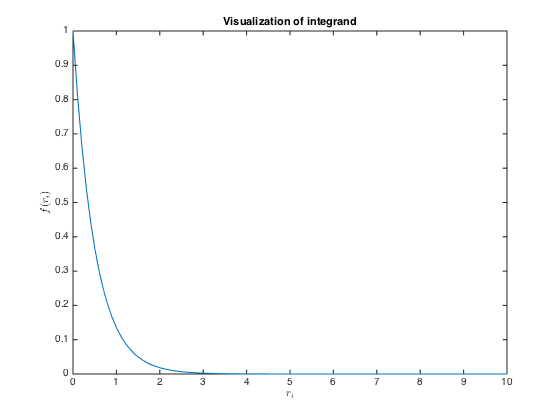
\includegraphics[width=90mm]{integrand.png} 	
	\captionof{figure}{The single-particle wave function $e^{-\alpha r_i}$.}
	\label{fig:integrand}
\end{center}
The function \verb@gauleg@ to calculate the weights and mesh points using Legendre polynomials has been provided. All we have to do is to call this function and go through a 6-dimensional nested \verb@for@-loop to calculate the sum which approximates the integral. 






\subsubsection{Gauss-Laguerre quadrature}
In using Legendre polynomials our originally infinite limits had to be approximated by finite ones. Our integral in Eq. (\ref{eq:correlationenergy}) can be rewritten with spherical coordinates to better deal with the infinite limits. Then the integral in becomes

\begin{equation}\label{eg:gaulag}
	I = \int    r_1^2 r_2^2 \frac{e^{- 2 \alpha (r_1 + r_2)}}{r_{12}} \sin \theta_1 \sin \theta_2 \mathrm{d}r_1  \mathrm{d}r_2 \mathrm{d}\theta_1 \mathrm{d}\theta_2 \mathrm{d}\phi_1\mathrm{d}\phi_2,
\end{equation}
where $r_i \in [0,\infty]$, $\theta_i \in [0,\pi]$ and $\phi_i \in [0, 2\pi]$, with

\begin{equation*}
	\frac{1}{r_{12}}= \frac{1}{\sqrt{r_1^2+r_2^2-2r_1r_2\cos(\beta)}},
\end{equation*}
where

\begin{equation*}
	\cos(\beta) = \cos(\theta_1)\cos(\theta_2)+\sin(\theta_1)\sin(\theta_2)\cos(\phi_1-\phi_2)).
\end{equation*}
The angular parts of the integral has finite limits and can be calculated using Legendre polynomials without having to have different limits in the analytical and numerical case. Great! The radial part of the integral however has limits [0,$\infty$), just as the Laguerre polynomials has. Thus we can use Laguerre polynomials with the weight function $W(x) = r^{\alpha} e^{-r}$ to calculate the radial parts of the integral. But first we need to do a variable change so that our integral is on the same form as the weight function. 

We substitute $r_i = u_i/2\alpha$ and $\mathrm{d}r_i = \mathrm{d}u_i/2\alpha$. In our case $\alpha = 2$, and the integral becomes

\begin{equation*}
	I = \frac{1}{1024} \int_0^{\pi} \sin \theta_1 \sin \theta_2 \mathrm{d}\theta_1 \mathrm{d}\theta_2 
	\int_0^{2\pi} \mathrm{d}\phi_1\mathrm{d}\phi_2
	\int_0^{\infty}   \mathrm{d}u_1  \mathrm{d}u_2 u_1^2 u_2^2 \frac{e^{- (u_1 + u_2)}}{r_{12}}.
\end{equation*}
Locating the part of the integral that represents the weight function $W(x)$ we see that the integral becomes

\begin{equation*}
	I = \frac{1}{1024} \int_0^{\pi} \sin \theta_1 \sin \theta_2 \mathrm{d}\theta_1 \mathrm{d}\theta_2 
	\int_0^{2\pi} \mathrm{d}\phi_1\mathrm{d}\phi_2
	\int_0^{\infty}   \mathrm{d}u_1  \mathrm{d}u_2 \frac{W(u_1) W(u_2)}{r_{12}}.
\end{equation*}
Thus 

\begin{equation*}
	g(u_1, u_2, \theta_1, \theta_2, \phi_1, \phi_2) = \frac{\sin \theta_1 \sin \theta_2}{r_{12}}.
\end{equation*}
The function \verb@gauss_laguerre@ to calculate the weights and mesh points of the radial parts of the integral has been provided. Again all we have to do is to call \verb@gauss_laguerre@ for the radial part, and \verb@gauleg@ for the angular parts, and go through a 6-dimensional nested \verb@for@-loop to calculate the sum which approximates the integral. 





\subsection{Monte Carlo}
The Monte Carlo method is a statistical simulation method which can be used for systems that are described by their probability distribution functions (PDFs). The Monte Carlo method proceeds by random samplings from the PDF. The final result is taken as an average over the number of simulations, and multiplied with the Jacobi determinant of the change of variables. With the limits $a$ and $b$, we change variables 
\begin{equation}
	r_{i,j} = a - (b-a)x_{i,j};\,i=1,2;\,j=1,2,3,
\end{equation}
where $x_{i,j}$ is a uniformly distributed random number between 0 and 1.
The Jacobi determinant for this is $(b-a)^6$, as we have 6 variables.
We solve the integral as it appears in eq.~(\ref{eq:cartesian}) with $x_{i,1} = x_i$, $x_{i,2} = y_i$, $x_{i,3} = z_i$, and $\alpha=2$. With this method we go from 6 nested \verb@for-loops@ to only one.

To get better precision we also run the Monte Carlo method by using importance sampling. For this case we return to spherical coordinates as it is given in eq.~(\ref{eg:gaulag}). The PDF of $r_i$ is given by
\begin{equation}
	P(r_i)=4\mathrm{e}^{-4r_i},
\end{equation}
so we want to use exponentially distributed random numbers. This is done by changing variables as follows
\begin{align*}
	r_i &\rightarrow -\frac{1}{4}\ln(1-x_i) \\
	\theta_i &\rightarrow \pi x_i \\
	\phi_i &\rightarrow 2\pi x_i,
\end{align*}
where $x_i$ is a random number between 0 and 1.
The Jacobi determinant is then given by $(1/4)^2\times\pi^2\times(2\pi)^2 = \pi^4/4$.

Lastly, we calculate the variance, 
\begin{equation}\label{eq:variance}
	\sigma^2 = \int\limits_{-\infty}^{\infty}\mathrm{d}xP(x)(x-\mu)^2 = \langle x^2\rangle-\langle x\rangle^2,
\end{equation}
which gives a measure of how far our set of points are separated.


\section{Results}
The results for the various methods are collected here with three leading digits:

\begin{center}
\begin{tabular}{ l l l l l}\hline
	Method 									& N	 				&I			&$\sigma$				& $t$ (s) \\ \hline
	Gauss-Legendre 							& 25 					& 0.196		& -						& 50 \\
	Gauss-Laguerre 							& 25					& 0.192		& -						& 38 \\
	Monte Carlo 								& 5 $\cdot 10^7$ 		& 0.197		& 7.00147 $\cdot 10^{-3}$		& 23 \\
	Monte Carlo*					 			& 1 $\cdot 10^6$		& 0.193		& 1.73337 $\cdot 10^{-2}$		& 0 \\
	\hline
\end{tabular}
\end{center}
where * denotes Monte Carlo method with importance sampling. The $N$ values given here are the minimal values we found to give satisfying results. The exact solution with three leading digits is 0.193.

The result from a run of the code can be seen in the file \verb@selected_results.txt@.




\section{Conclusions}

From the results it is obvious that Monte Carlo with importance sampling is the preferred method. The result is excellent and the time spent to run the code is incredibly low.

The result from the regular Monte Carlo method is not very impressive. For lower $N$ the result becomes too small, and for larger $N$ the code takes too long to give a result.

The time it takes to run Gauss-Legendre and Gauss-Laguerre increases rapidly with $N$, making these methods unbearably slow. Testing out different values of $N$ showed that the result from Gauss-Legendre was very unstable with changing $N$, while Gauss-Laguerre improved for larger $N$. But the improvement in precision was low compared to the increase in time, so we limited the calculation to $N = 25$. 





\section{List of codes}

The codes developed for this project are:\\

\noindent \verb@main.cpp@ -- main program, C++

\noindent \verb@plotting.m@ -- plotting program, MATLAB

\end{multicols}

\end{document}
